% Drawing 154/08-12 -- folder 154, batch 08, archive page 156 (PDF page 157).
% Transcription: en bas à gauche, un dessin en couleur : deux droites orange qui se croisent en un point $s$ ; une droite vert clair en tirets $D_0$, fléchée, passant par $s$, entre deux droites vert clair $D'$ (au-dessus, fléchée $\omega^{*}$) et $D$ (au-dessous) ; les orientations $\alpha^{*}$ (rotation) et $\beta^{*}$ (flèche brune transverse) ; le triangle marqué $T$ sous le croisement
% Kind: two crossing lines at s with D_0 dashed through s between D' and D; orientations. Method 2 (schematic redraw from the facsimile). Status: ok.
% Notes: Bottom left, a colour drawing: two orange lines crossing at a point s; a light green dashed line D_0, arrowed, through s, between two light green lines D' (above, arrowed omega*) and D (below); the orientations alpha* (rotation) and beta* (arrow) at s, a thick arrow along D_0. The many similar small drawings in the rest of the page are not covered by this mark. Read from the page view.
% Coordinates: 1 unit = 1 mm = 1/100 of the crop width (bbox in page fractions: [0.125, 0.31, 0.302, 0.406]).
% Redrawn by Claude (claude-opus-5-5), issue #73, 2026-11-07; not checked by a human; not compiled (no TeX in the session).
% Revised by Claude (claude-opus-5-5) 2026-11-09 (issue #128) after Michel's check: vertices snapped to exact intersections (drawn points on their lines, meeting ends on the stroke they meet, near-concurrent lines through one computed point, curve ends on their rim); labels at \small as in folder 80 batch 3. Status: ok.
% Rights: reproduces part of the work -- behind RENDER_TRANSCRIPTS, never published by itself.
\documentclass[tikz,border=3pt]{standalone}
\usepackage{amsmath,amssymb}
\usetikzlibrary{patterns,arrows.meta}
\tikzset{Or/.style={orange!90!black}, Ye/.style={yellow!80!orange}, Lg/.style={green!60!black!70}, Dg/.style={green!45!black}, Br/.style={brown!80!black}, Rd/.style={red!85!black}, Bl/.style={blue!70!black}, Gy/.style={black!40}, pencil/.style={black!45}, struck/.style={black!35}, mark/.style={circle,draw,inner sep=1.3pt}, pt/.style={circle,fill,inner sep=0.9pt}, opt/.style={circle,draw,fill=white,inner sep=1.1pt}}
\colorlet{Or}{orange!90!black}\colorlet{Ye}{yellow!80!orange}\colorlet{Lg}{green!60!black!70}\colorlet{Dg}{green!45!black}\colorlet{Br}{brown!80!black}\colorlet{Rd}{red!85!black}\colorlet{Bl}{blue!70!black}\colorlet{Gy}{black!40}
\begin{document}
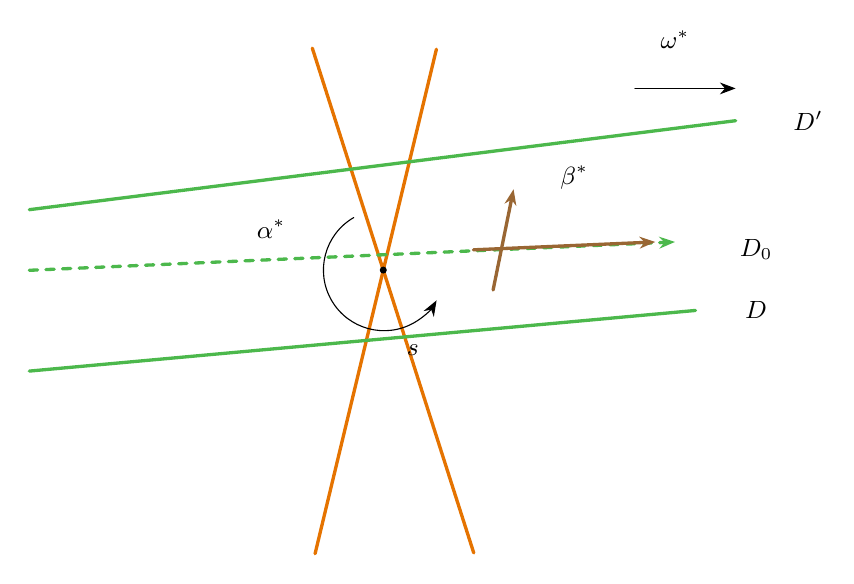
\begin{tikzpicture}[x=1mm,y=1mm,line cap=round,line join=round,font=\scriptsize]
\draw[Or,very thick] (38.54,-10.29) -- (59.04,-74.39);
\draw[Or,very thick] (54.3,-10.42) -- (38.89,-74.49);
\node[pt] at (47.55,-38.47) {};
\node[inner sep=1pt] at (51.3,-48.7) {\small $s$};
\draw[Lg,very thick] (2.6,-30.8) -- (92.3,-19.5);
\node[inner sep=1pt] at (101.5,-19.5) {\small $D'$};
\draw[-{Stealth[length=2mm]}] (79.5,-15.4) -- (92.3,-15.4);
\node[inner sep=1pt] at (84.6,-9.2) {\small $\omega^{*}$};
\draw[Lg,dashed,very thick,-{Stealth[length=2mm]}] (2.6,-38.5) -- (84.6,-34.9);
\node[inner sep=1pt] at (94.9,-35.9) {\small $D_0$};
\draw[Br,very thick,-{Stealth[length=2mm]}] (59,-35.9) -- (82.1,-34.9);
\draw[Lg,very thick] (2.6,-51.3) -- (87.2,-43.6);
\node[inner sep=1pt] at (94.9,-43.6) {\small $D$};
\draw[Br,very thick,-{Stealth[length=2mm]}] (61.5,-41) -- (64.1,-28.2);
\node[inner sep=1pt] at (71.8,-26.7) {\small $\beta^{*}$};
\draw[-{Stealth[length=2mm]}] (43.8,-31.8) arc[start angle=120, end angle=330, x radius=7.7, y radius=7.7];
\node[inner sep=1pt] at (33.3,-33.3) {\small $\alpha^{*}$};
\end{tikzpicture}
\end{document}
